\section{Evaluation}
\label{sec:eval}
In this section we evaluate the performance of the proposed ETA system \texttt{ACETA}. In particular we focus on the training time, inference time, accuracy, and performance breakdown of the different steps. First, we cover the experiment background and methodology for executing the comparisons. Then we discuss general performance improvements made in \texttt{ACETA} relative to the \texttt{Joy} baseline. After addressing general improvements, we cover each of the aforementioned performance metrics in detail for each of the models tested.  

\subsection{Experiment Platform and Methodology}
We perform all testing for \texttt{ACETA} on a commodity workstation with Intel x86 processors to resemble the real-world uCPE setting. The Intel Distribution for Python is used in an Anaconda environment for all programming, with all applicable additional packages coming via the Intel channel. The detailed hardware and software specifications are listed in Table \ref{tbl:platform}. We use the \texttt{CICAndMal2017} dataset \cite{cicandmal2017}, provided by the University of New Brunswick, for training and testing in all comparisons . In addition to benign flows, this dataset contains four categories of malware: adware, ransomware, scareware, and SMS malware, with samples coming from 42 unique malware families. Comparing the baseline with \texttt{ACETA} first involves randomly splitting subsets of the processed data for training and testing, providing one sample from each of the malware families per subset, along with many more benign samples. The subsets are partitioned, and then saved to separate files to be shared by the baseline and \texttt{ACETA} for level comparison results. We use the standard Python time library for the timing of model training, and we measure the accuracy by using the labels of 0 and 1 for benign and malicious samples respectively. Performance statistics are gathered using the generic cProfiling Python utility, along with the kcachegrind tool \cite{kcachegrind} to process and present the data. 

\begin{table}[h!]
\scriptsize
\centering
\caption{Experiment Platform Specification}
\begin{tabular}{|c|c|}
  \hline
  Item  & Specification \\
  \hline\hline
  CPU &  Intel Core i5-8600k 6 cores @ 3.60GHz\\
  \hline
  Memory & 16 GB DDR4 @ 2667MHz\\
  \hline
  HDD & 1TB @ 7200RPM\\
  \hline
  Software & Intel DAAL v0.2019.3\\
  \hline
  & Intel OpenVINO v2019.1.144\\
  \hline
  & Anaconda v5.3.0 \\
  \hline
  Host OS & Ubuntu 16.04 Desktop\\
  \hline
\end{tabular}
\label{tbl:platform}
\end{table}

\subsection{Performance Results}
The baseline raw to processed data pipeline takes on average 33.7 minutes for completion. Given this result, we begin to implement strategies to accelerate the pipeline. Initial data processing optimizations such as list comprehensions, string formatting, accelerated conditional processing using try-catch, and using Numpy arrays instead of Python lists improve the average performance to 30.1 minutes, a speedup of 8.3\%. Multiprocessing the initial data processing with \texttt{Joy}, and also the feature analysis result in an average performance of 23.2 minutes, a speedup of 31.2\% relative to the baseline. Next, we exploit the ujson library as a drop-in replacement for the standard JSON library, resulting the process to take only 17.8 minutes, a cumulative speedup of 47.2\%.

\subsubsection{Training Time}
In the model creation phase of \texttt{ACETA}, the user has the option to select which type of model to train and save. Currently, the model options are logistic regression, decision forest, support vector machine, and an artificial neural network. The baseline version of the code uses Scikit-learn library for the models, while \texttt{ACETA} uses DAAL, with both versions' models using identical parameter settings. The log scale training time of each of the models for the two versions are shown in figure \ref{figure:training-time}. For all of the models except the neural network, the \texttt{ACETA} versions outperform the original by several factors: 10x faster for logistic regression, 3.25x faster for decision forest, and 31x faster for SVM. A 100-epoch neural network comparison results in the \texttt{ACETA} version being around twice as slow as the original. One possible reason for this inconsistency is that the original model uses a deprecated, Scikit-learn neural network API, whereas \texttt{ACETA} uses an Intel Python distribution Keras \cite{keras} model. DAAL offers low level APIs, similar to standard TensorFlow, to design neural networks piece-by-piece, but for the sake of simplicity Keras is used in our implementation. However, it is also worth noting that optimizing this TensorFlow based model, using Intel's OpenVINO deep learning framework \cite{openvino}, results in a faster inference time relative to the baseline neural network.

\begin{figure}[h!]
	\centering
	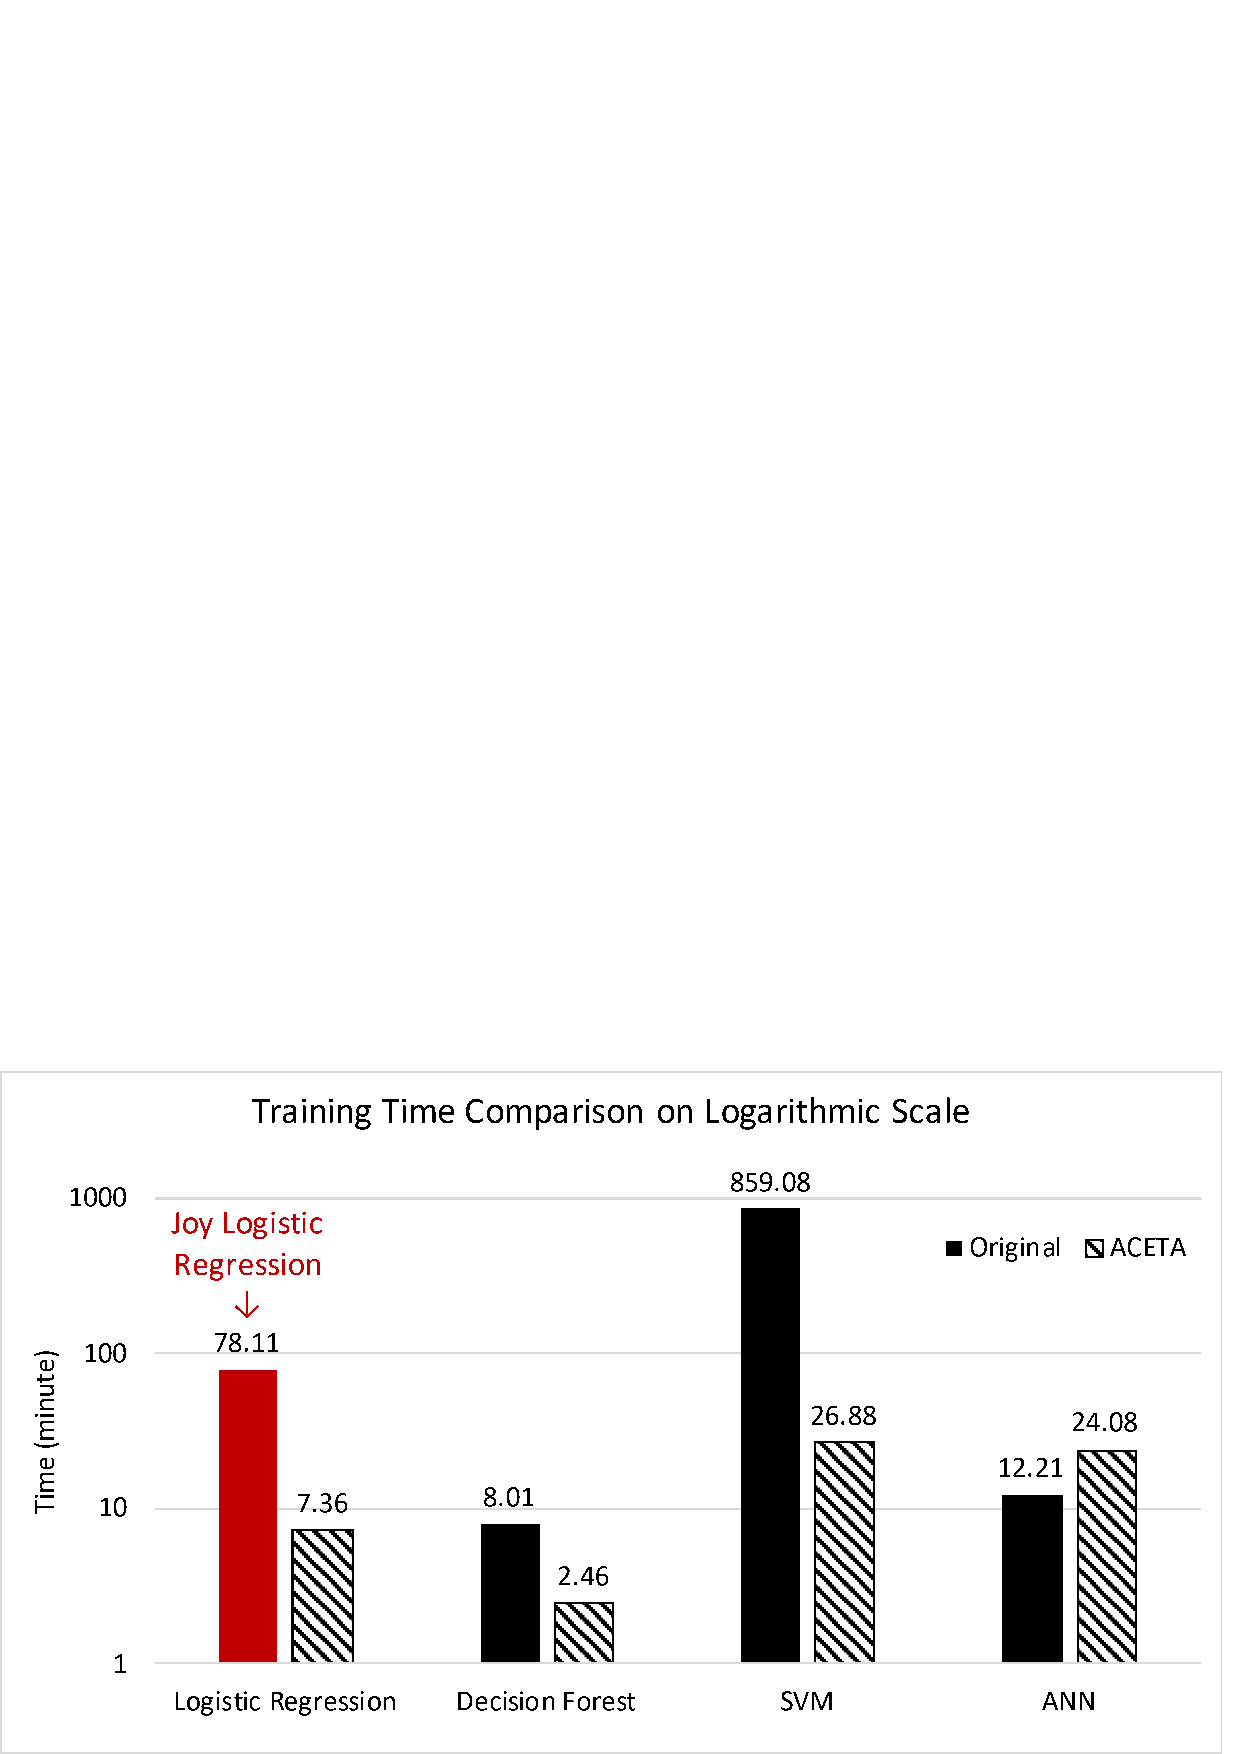
\includegraphics[width=3.3in]{./fig/training-log.pdf}
	\caption{Training Time Comparison on Logarithmic Scale}
	\label{figure:training-time}
\end{figure}

\subsubsection{Inference Time}
In addition to improving training performance, \texttt{ACETA} also performs significantly faster for inference. Figure \ref{figure:inference-time} presents the time comparisons for each model on an identical dataset. The baseline models all complete in roughly 925 milliseconds, compared to the majority of \texttt{ACETA} models taking only 20 milliseconds, a 46x improvement. The only model to underperform is the \texttt{ACETA} ANN, taking about 1.49 seconds to complete its inference (not shown in Figure \ref{figure:inference-time}). However, by optimizing the \texttt{ACETA} Keras/TensorFlow ANN model with Intel OpenVINO, the optimized model inference takes only 30 milliseconds, on the order of the other \texttt{ACETA} models, while retaining the same accuracy as its unoptimized counterpart. 

\begin{figure}[h!]
	\centering
	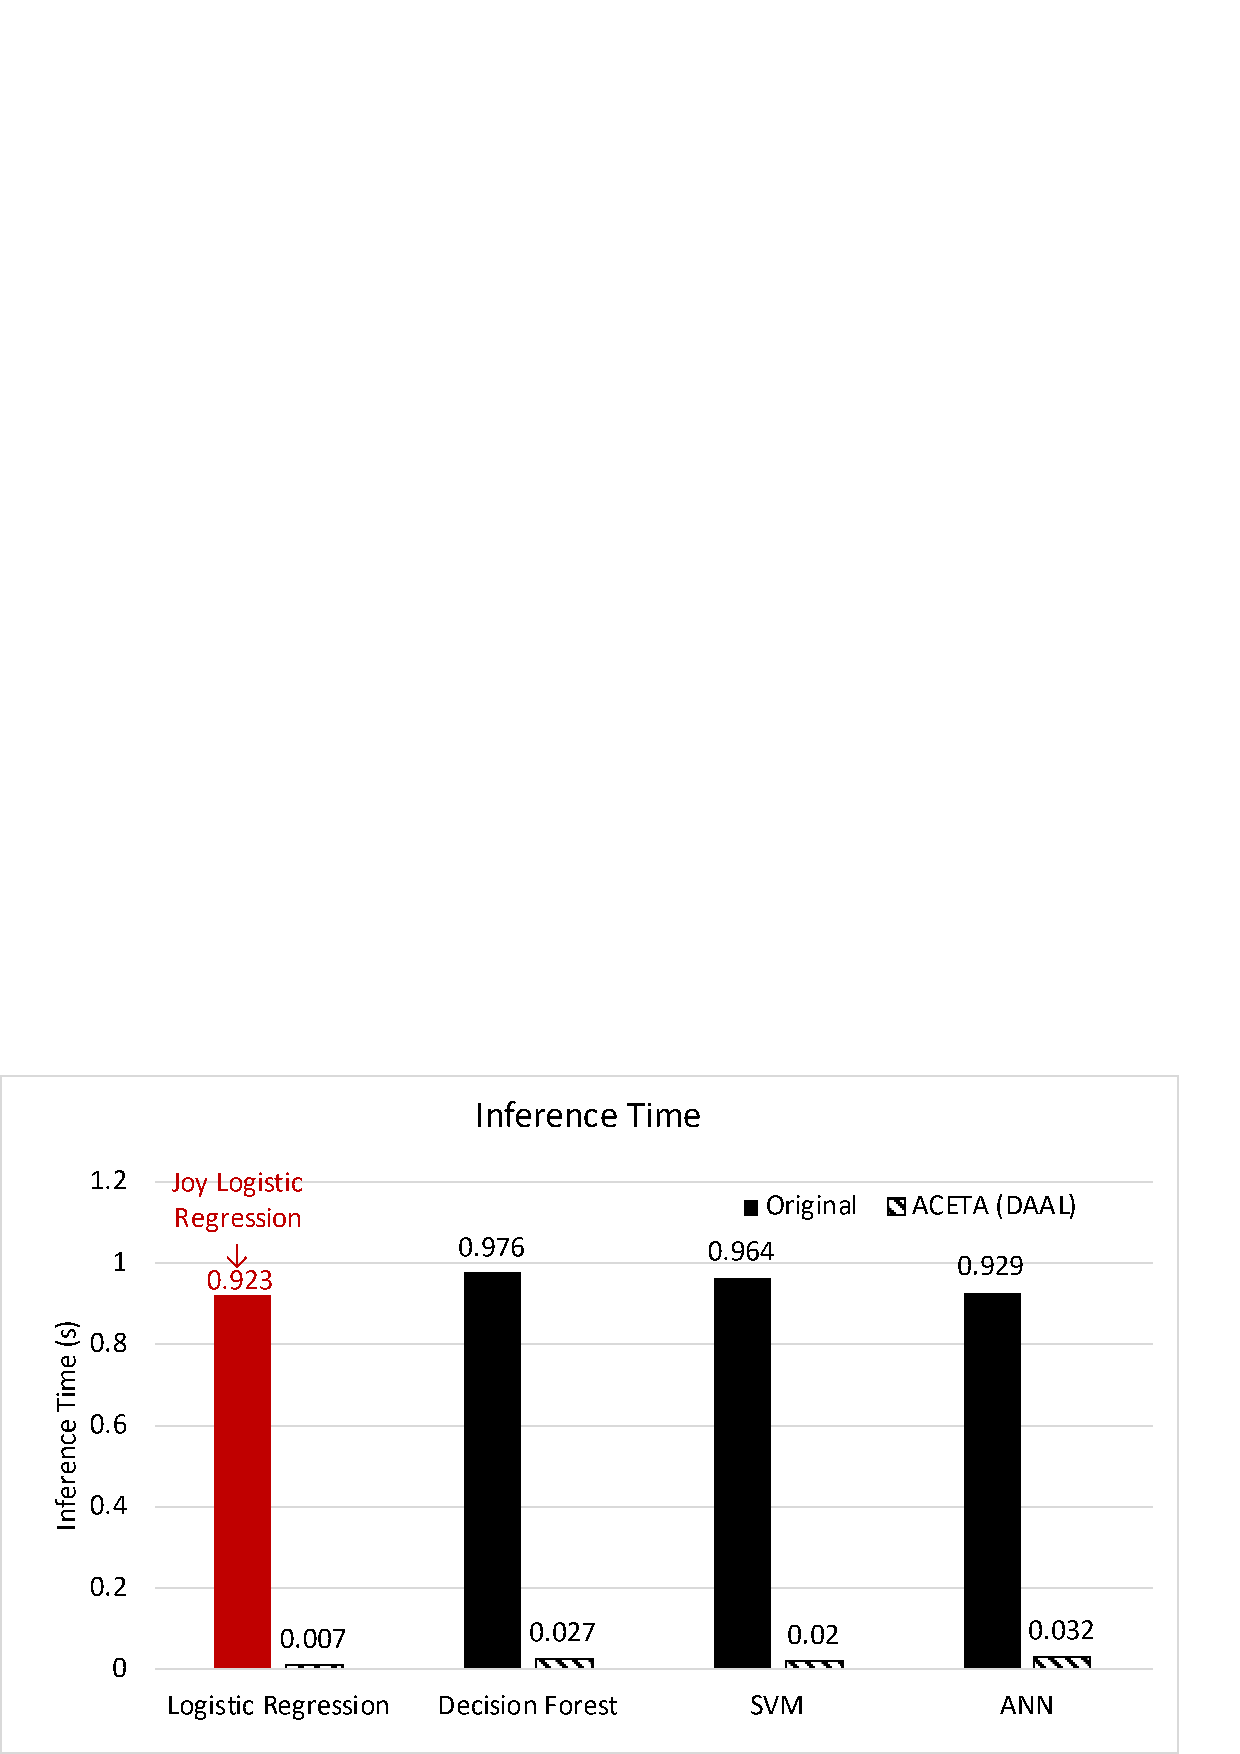
\includegraphics[width=3.3in]{./fig/inference-time.pdf}
	\caption{Inference Time Comparison}
	\label{figure:inference-time}
\end{figure}

\subsubsection{Accuracy}
Figure \ref{figure:training-accuracy} shows accuracy comparisons for model training while Figure  \ref{figure:inference-accuracy} demonstrates inference accuracy on an identical test dataset immediately after model training. With each of the models, the performance shows very little difference between the baseline and \texttt{ACETA}. At most, \texttt{ACETA}'s accuracy is ~2.5\% lower for logistic regression training, but on average the difference is around a single percent. In the case of the decision forest classifier, the \texttt{ACETA} version even outperforms the slower, baseline model. This data, in addition to the training and inference time results, provides significant support for the use of DAAL as an alternative to the standard machine learning libraries.

\begin{figure}[h!]
	\centering
	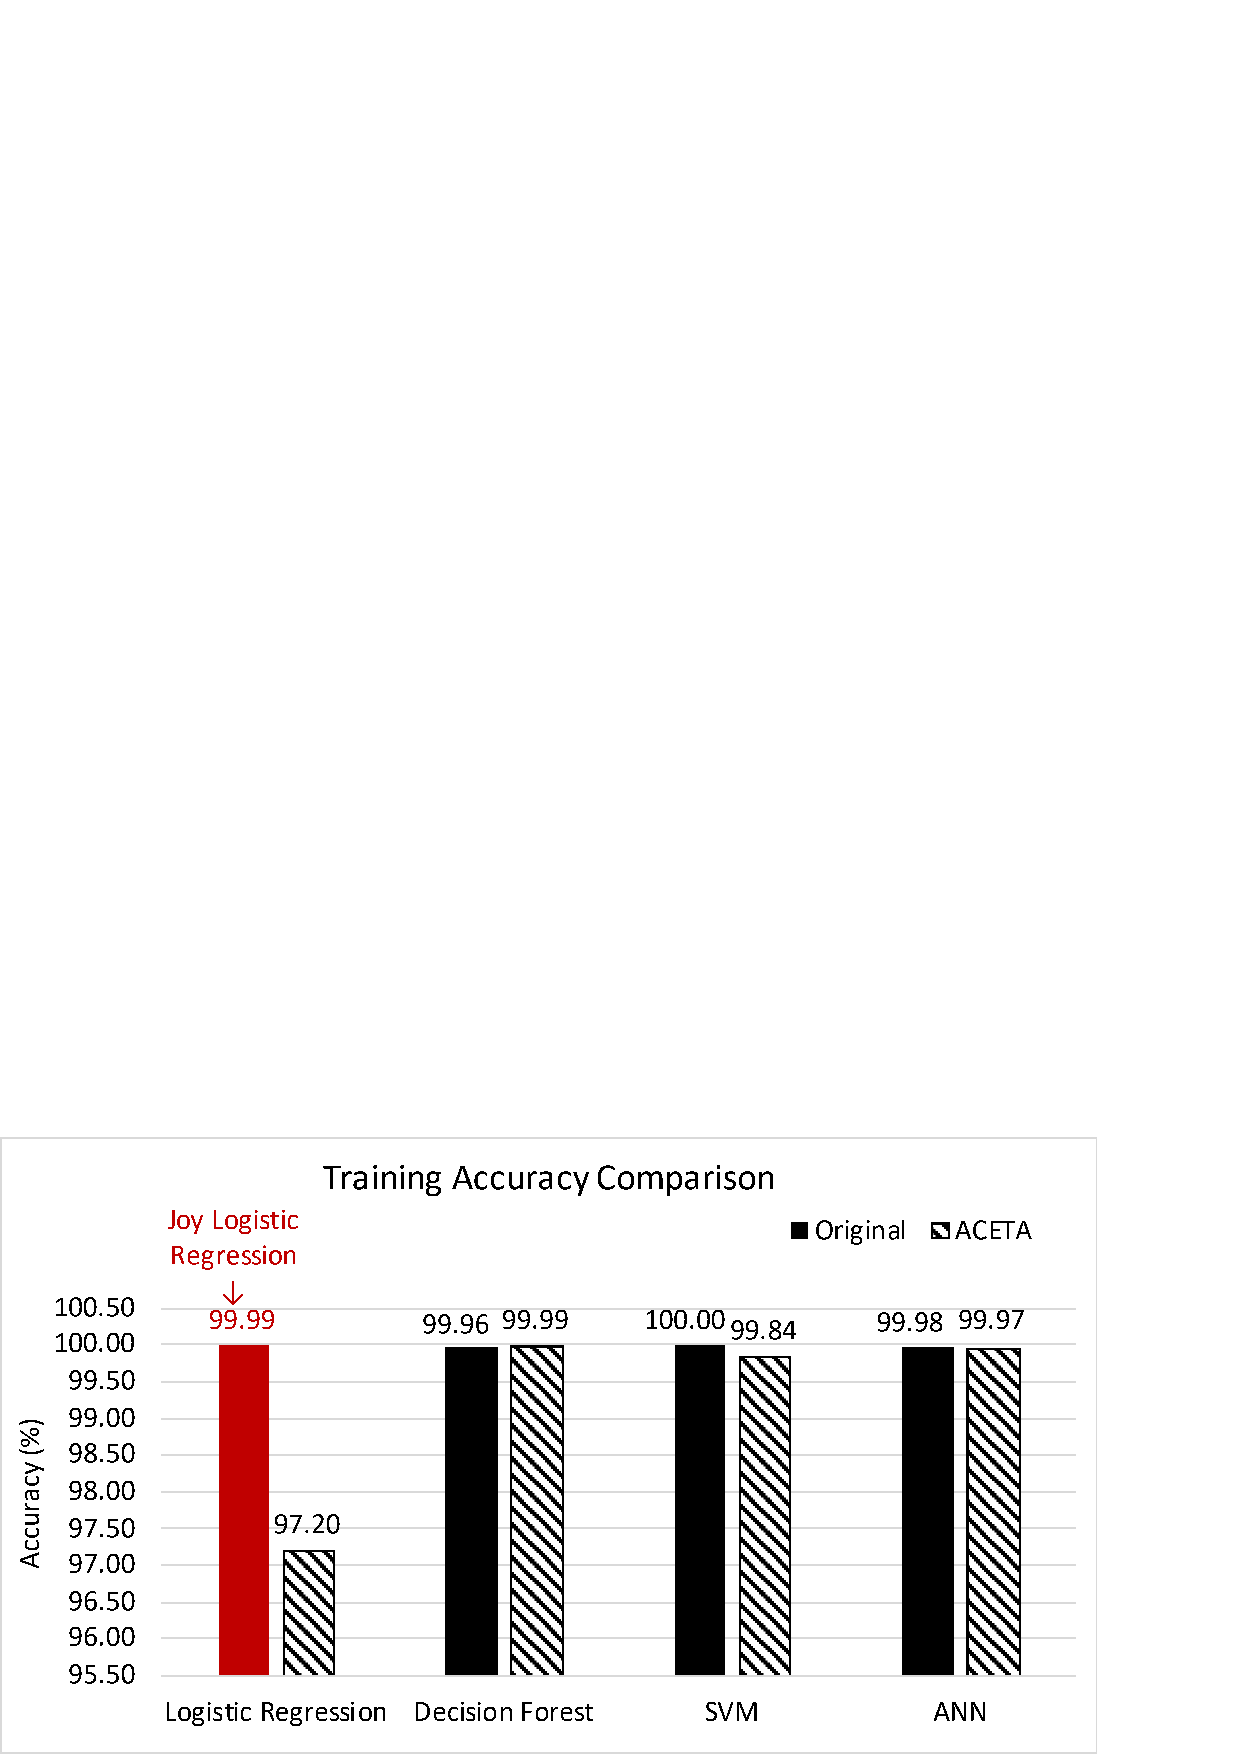
\includegraphics[width=3.3in]{./fig/training-accuracy.pdf}
	\caption{Training Accuracy Comparison}
	\label{figure:training-accuracy}
\end{figure}

\begin{figure}[h!]
	\centering
	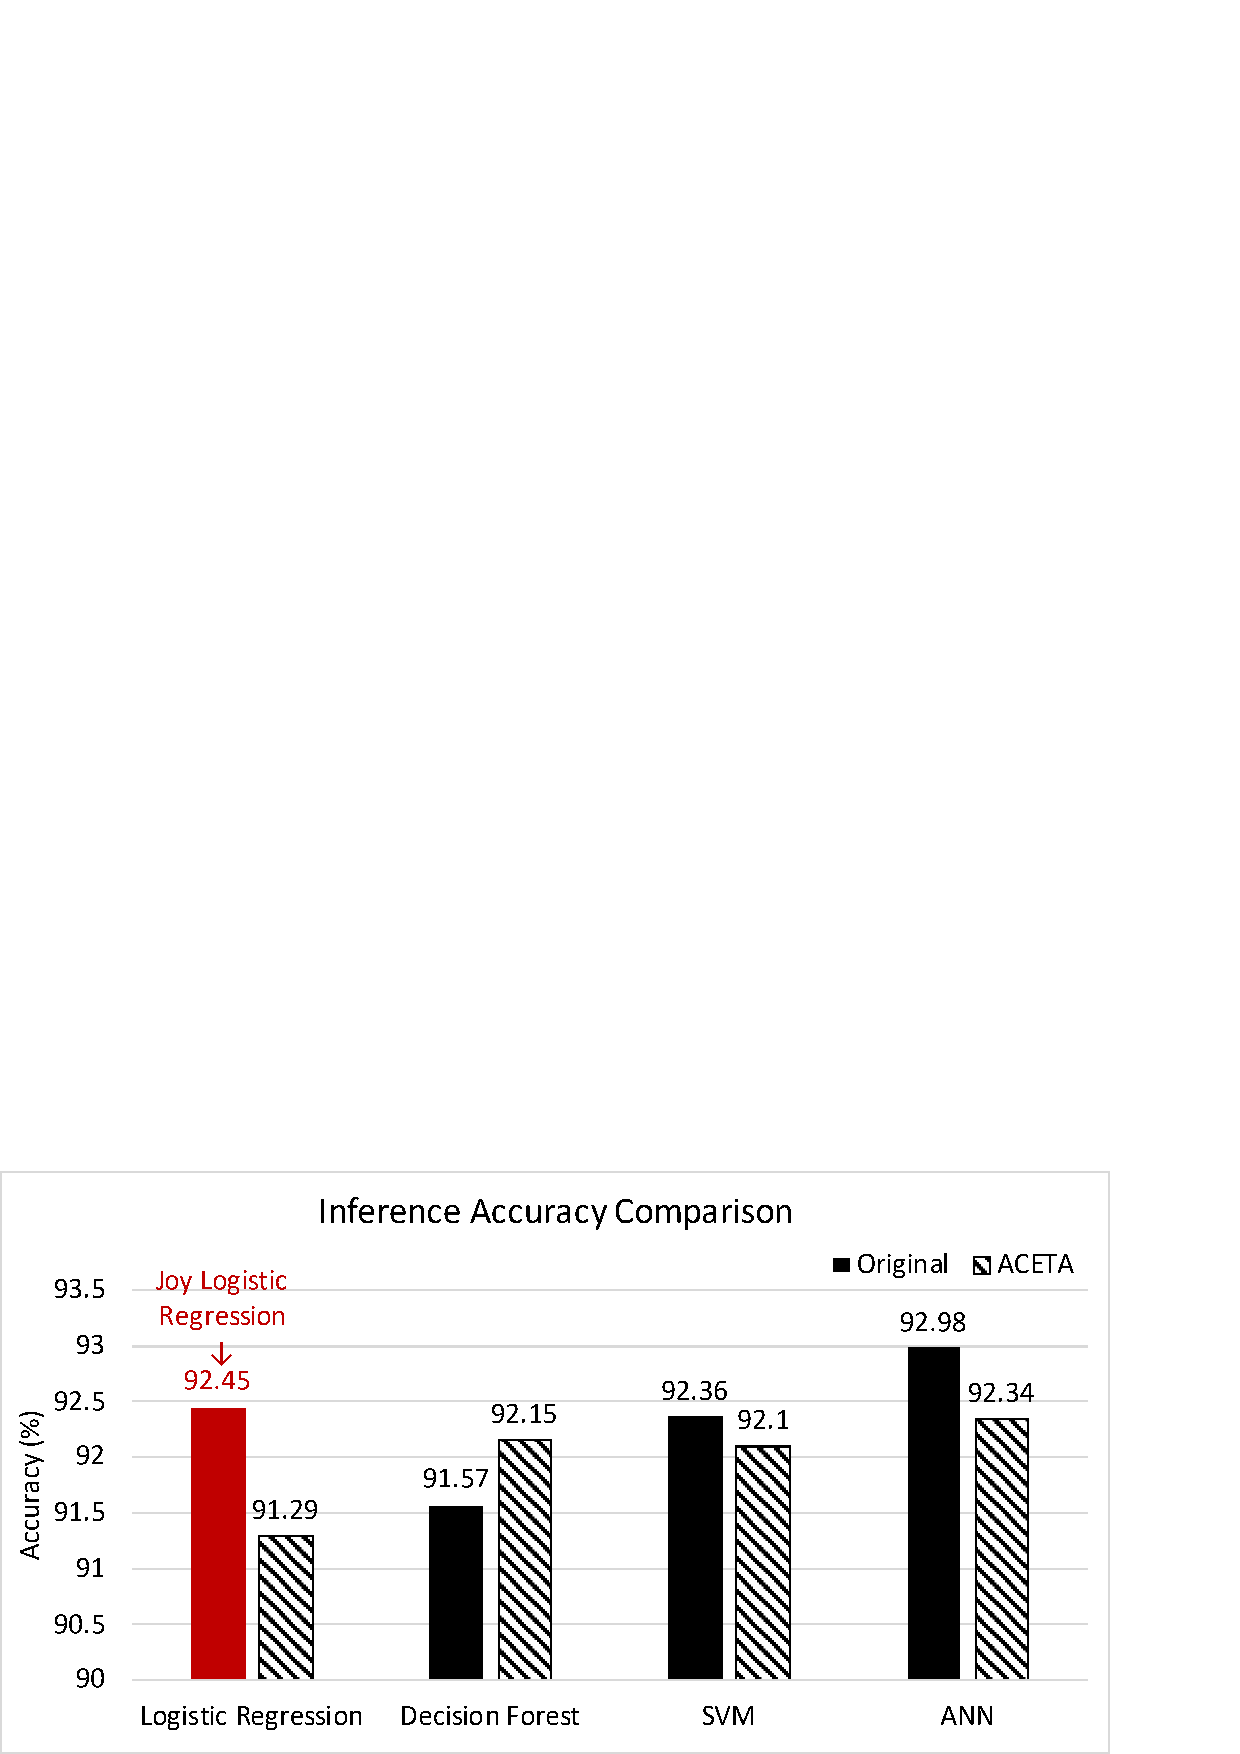
\includegraphics[width=3.3in]{./fig/inference-accuracy.pdf}
	\caption{Inference Accuracy Comparison}
	\label{figure:inference-accuracy}
\end{figure}

\subsubsection{Performance Breakdown}
We leverage the cProfiling utility to track and save the cumulative time the program spends in each of its functions. Using kcachegrind \cite{kcachegrind}, we visualize the data to locate the major hotspots within the training of each of the models. Figure \ref{figure:breakdown} displays this breakdown separated into three categories: training, data preparation, and other. For the majority of the models, the training of the models occupies the biggest percentage of time, which is to be expected. With the acceleration of DAAL and OpenVINO, the \texttt{ACETA} versions receive a great decrease on the overall training time percentage. One interesting observation is the training time percentage of the \texttt{ACETA} decision forest: it is not the most time consuming part of the algorithm. This can be explained by this model being by far the fastest to complete training, so the data processing and overhead inevitably occupy larger percentages of time. With both logistic regression and SVM showing a similar breakdown, the other interesting comparison is between the original and \texttt{ACETA} ANN. As mentioned earlier, the \texttt{ACETA} ANN version uses Keras \cite{keras}, which provides a high-level API to create TensorFlow models. This supports the measured \texttt{ACETA} ANN breakdown that shows a larger percentage of time, 32.3\%, being consumed by other tasks, other being the lump sum of any additional overhead. This irregularity explains at least in part the performance disparity between the baseline and \texttt{ACETA} ANN versions.

\begin{figure}[h!]
	\centering
	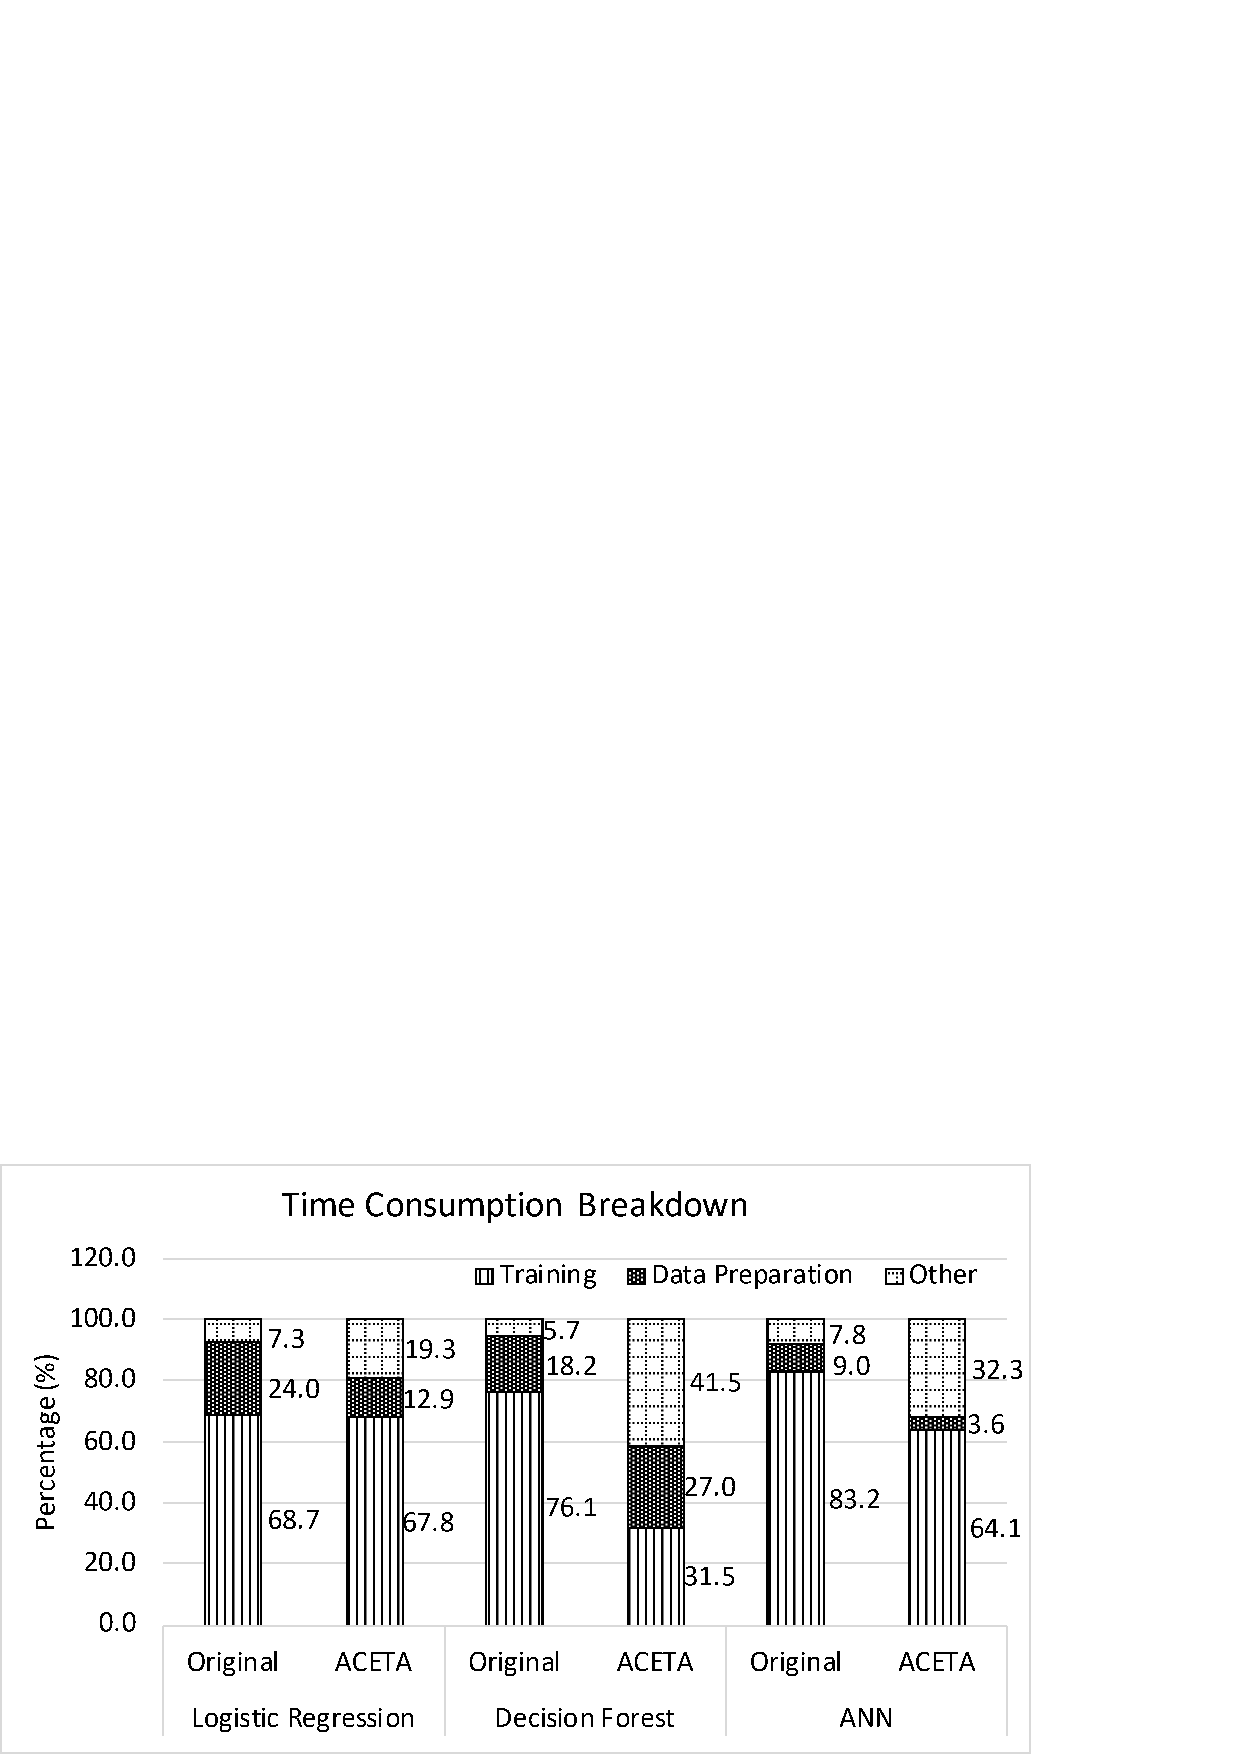
\includegraphics[width=3.3in]{./fig/perf-breakdown.pdf}
	\caption{Time Consumption Breakdown}
	\label{figure:breakdown}
\end{figure}
